\documentclass[en]{./../../common/SurferDesc}%%%%%%%%%%%%%%%%%%%%%%%%%%%%%%%%%%%%%%%%%%%%%%%%%%%%%%%%%%%%%%%%%%%%%%%
%
% The document starts here:
%
\begin{document}
\footnotesize
% Weltrekordfl�chen

%%% 1.Tafel

%%%%%%%%%%%%%%%%%%%%%%%%%%%%%


\begin{surferPage}
  \begin{surferTitle}A 7-gon-symmetric Septic\end{surferTitle}   \\
    This surface which looks like a star has degree $7$.  
    Until recently its number of singularities, $84$, was still the
    maximum number of real singularities known for septics;
    only in 2004, Oliver Labs improved this world record to $99$.
  
  
 The three cushions which one can see in the interactive picture, 
    are caused by the use of Chebychev polynomials, similar to the Chmutov
    Octic. 
    In fact, this star shaped surface is another variant of Chmutov's surfaces.
    Here, the plane curve $T_d(x)+T_d(y)$ was replaced by a regular $7$-gon
    $S_7(x,y)$: 
   \[S_7(x,y) + \lambda \cdot T_d(z) = 0,\]
    for a suitably chosen $\lambda\in\RR$. 
    \vspace*{-0.3em}
    \begin{center}
      \begin{tabular}{c@{\qquad}c}
        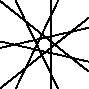
\includegraphics[height=1.5cm]{./../../common/images/labsseptic1.pdf}
        &
        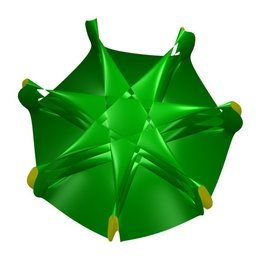
\includegraphics[height=1.5cm]{./../../common/images/septic_7eck_von_oben}
      \end{tabular}
    \end{center}
    \vspace*{-0.3em}   
   This variant of Chmutov's construction is provided by Duco van Straten. 


  \begin{surferText}
     \end{surferText}
\end{surferPage}



\end{document}
%
% end of the document.
%
%%%%%%%%%%%%%%%%%%%%%%%%%%%%%%%%%%%%%%%%%%%%%%%%%%%%%%%%%%%%%%%%%%%%%%%
